\begin{figure*}[htp!]
    \centering
    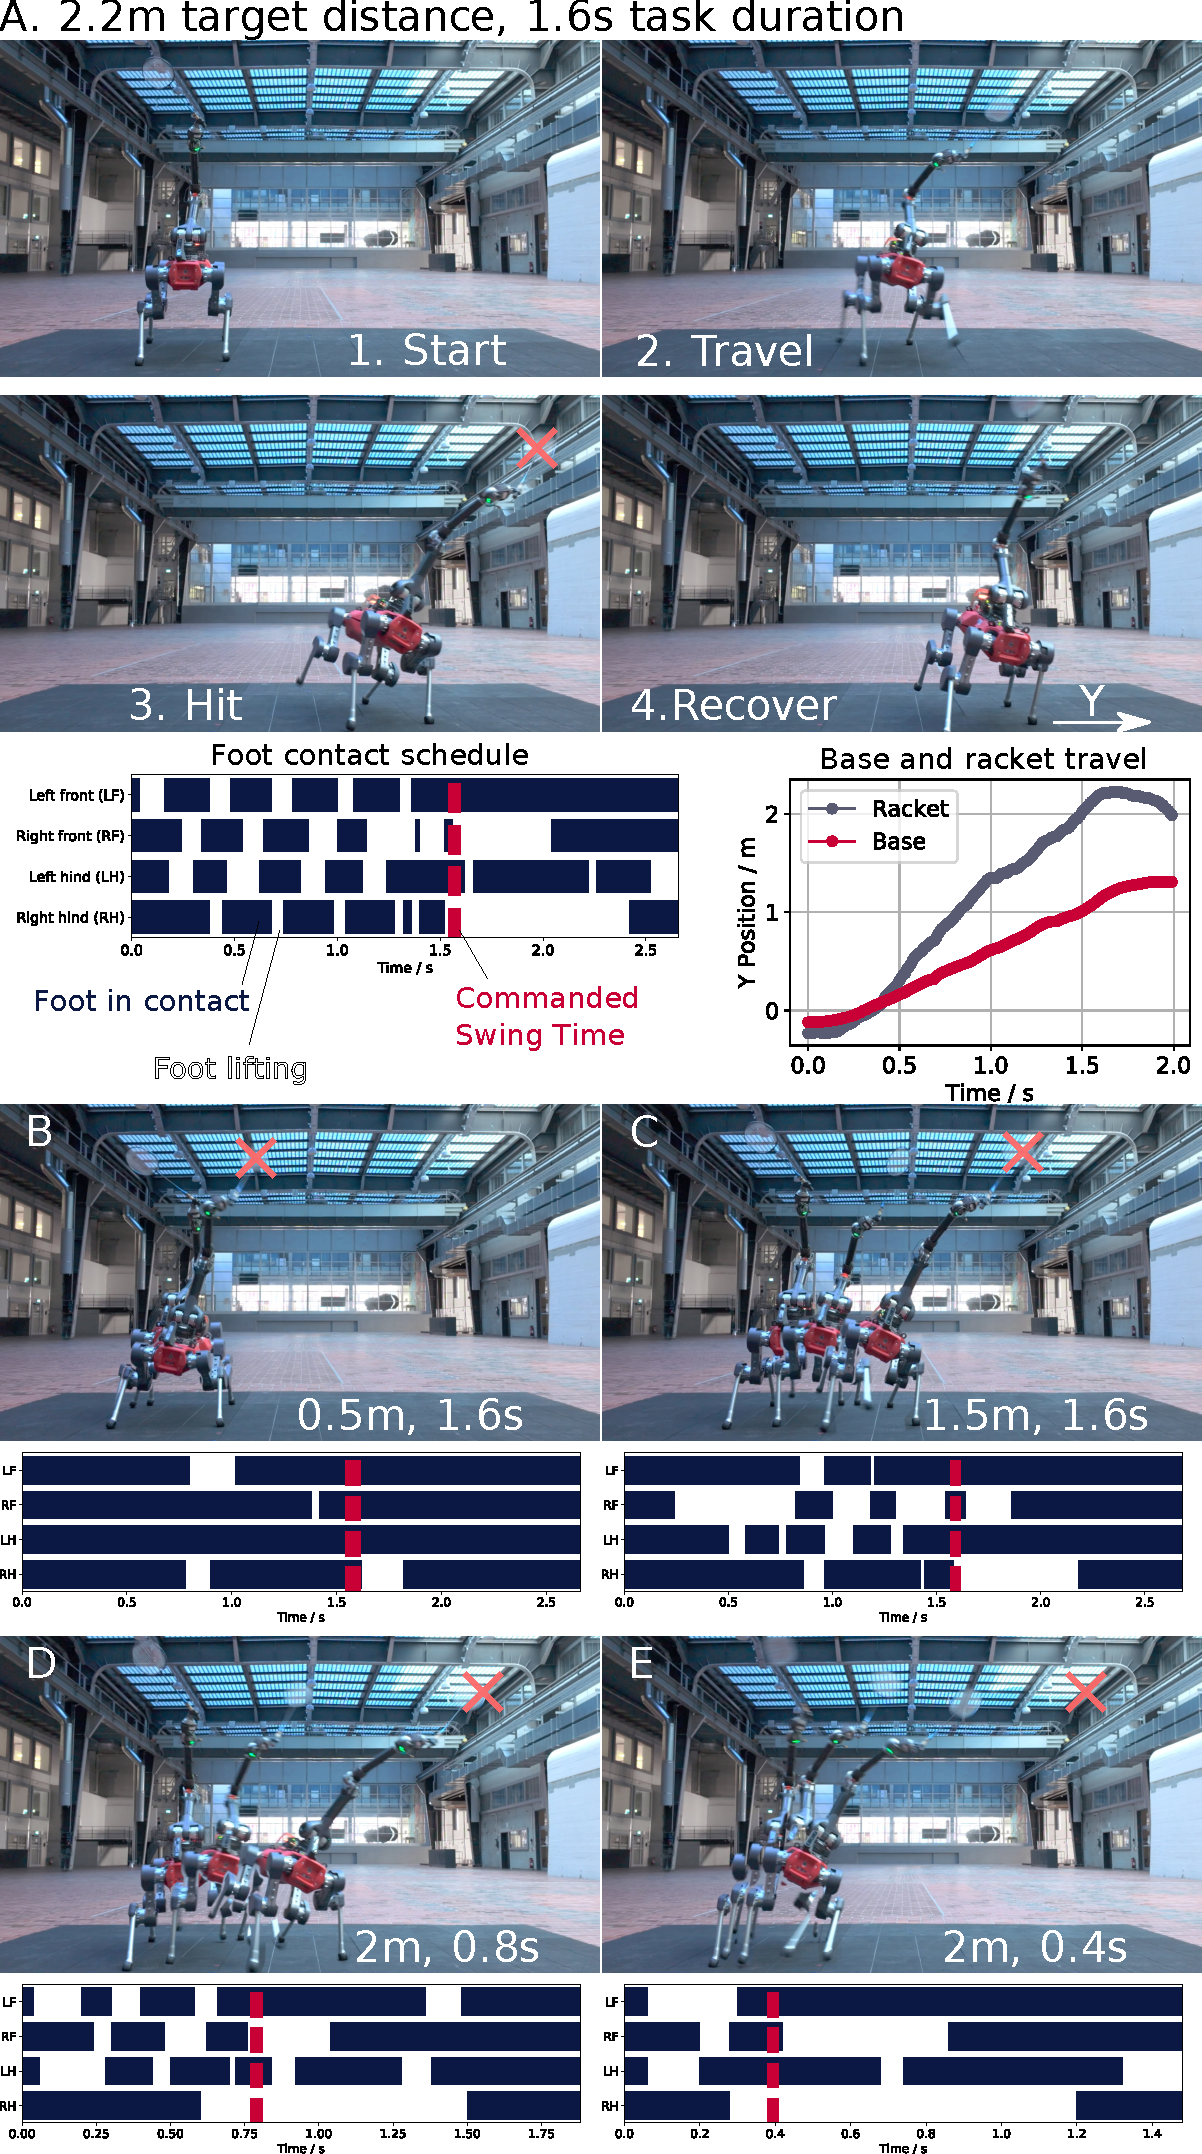
\includegraphics[height=0.77\textheight]{Figures/GaitAdaptation/gait_adaptation_compressed.pdf}
    \caption{\textbf{Gait adaptation based on distance and time urgency. (A)} The robot reaches targets \unit[2.2]{m} away from the starting base position in \unit[1.6]{s} using a galloping-like gait. Near the swing, the longer right foot lift phase and increased $y$-coordinate difference between the base and racket indicate a gait adjustment. \textbf{(B-C)} When targeting nearby positions, the robot barely lifts its feet. It steps to locomote when the target is out of reach. \textbf{(D-E)} Under tight time constraints, the control policy balances between maintaining safety and tracking the target accurately.}
    \label{fig:gait_adaptation}
    
    % \vspace{-1.5em}
\end{figure*}

% what's y axis
% initial position, hit position